\begin{center}
            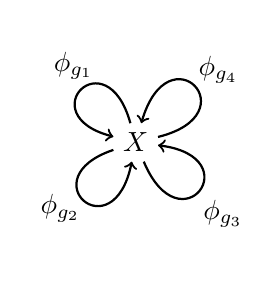
\begin{tikzpicture}
                \node at (0,0) (loop) {$X$};
                \begin{scope}[rotate= 55]
                    \draw[thick, <-] (loop) to [looseness=11, out=120,in=60,] node[above, xshift=-0.1cm] {$\phi_{g_1}$} (loop);
                \end{scope}
                \begin{scope}[rotate = 145]
                    \draw[thick, <-] (loop) to [looseness=15, out=120,in=60,] node[above, yshift=-0.4cm, xshift = -0.3cm] {$\phi_{g_2}$} (loop);
                    \begin{scope}[rotate = 80]
                        \draw[thick, <-] (loop) to [looseness=15, out=120,in=60,] node[above, yshift=-0.6cm, xshift = 0.3cm] {$\phi_{g_3}$} (loop);
                    \end{scope}
                \end{scope}
                \begin{scope}[rotate = 305]
                    \draw[thick, <-] (loop) to [looseness=12, out=120,in=60,] node[above, yshift=-0.1cm, xshift = 0.3cm] {$\phi_{g_4}$} (loop);
                \end{scope}
            \end{tikzpicture}
        \end{center}